\documentclass{JAC2003}


% This nonsense seems to be required to ensure that pdflatex processes this
% style correctly.
\ifx\pdfoutput\undefined
\else
\setlength{\paperwidth}{210mm}
\setlength{\paperheight}{296mm}
\setlength{\pdfpagewidth}{\paperwidth}
\setlength{\pdfpageheight}{\paperheight}
\fi

\usepackage{graphicx}       % Extended support for \includegraphics
\usepackage{tikz}           % Powerful drawing package, part of pgf

\usepackage{array}          % Improved array support
\usepackage{booktabs}       % Publication quality tables

\usepackage{mathptmx}       % Mathematical PostScript fonts
\usepackage{amsmath}        % General mathematical symbols
\usepackage{textcomp}       % Extra symbols

\usepackage{url}            % \url command for decent line breaks in urls
\usepackage{enumitem}       % For more control over list parameters.

\usetikzlibrary{matrix}             % Grid placement
\usetikzlibrary{positioning}        % Anchor placement support
\usetikzlibrary{calc}               % Coordinate calculations
\usetikzlibrary{shapes.geometric}   % cylinder
\usetikzlibrary{shapes.symbols}     % cloud
\usetikzlibrary{shapes.arrows}      % arrow shapes
\usetikzlibrary{shapes.multipart}
\usetikzlibrary{fit}                % Fitting outline to shape
\usetikzlibrary{shadows}

% Common TikZ definitions
\tikzset{
    % This seems a reasonably comfortable arrow shape
    >=stealth,
%
    % Used for creating an exact fit to an existing list of objects
    tight fit/.style={fit=#1, inner sep=0, line width=0},
%
    % Draws a reasonably sensible looking disk icon
    disk icon/.style={
        draw, thick, cylinder, shape border rotate=90,
        minimum width=1cm, minimum height=.75cm},
%
    % A moderate highlighting fill
    background fill/.style={fill=black!15},
    % A gentle highlighing fill
    highlight fill/.style={fill=green!60!blue!20},
    % A fill for highlighting an area of text
    text fill/.style={fill=orange!20, rounded corners},
    % A rather darker fill for shadows
    shadow fill/.style={fill=gray}}


% It's handy to have a foreground and background layer available.
\pgfdeclarelayer{background}
\pgfdeclarelayer{foreground}
\pgfsetlayers{background,main,foreground}



\hyphenpenalty 4000 % Tone down hyphenation


% For development when we don't want to spend the time required to render
% images, we can replace \includegraphics with the dummy below.
\newcommand{\dummyincludegraphics}[2][]{%
    $\backslash$\texttt{includegraphics}[\dots]\{#2\}}
\newcommand{\dummyinput}[1]{$\backslash$\texttt{input}\{#1\}}

% \def\includegraphics{\dummyincludegraphics}
% \def\input{\dummyinput}
% \renewcommand{\baselinestretch}{1.5}


\begin{document}
\title{A NEW FAST DATA LOGGER AND VIEWER AT DIAMOND:\\THE FA ARCHIVER}

\author{%
    M.G.~Abbott, G.~Rehm, I.S.~Uzun,
    Diamond Light Source, Oxfordshire, UK}

\maketitle

\begin{abstract}

At Diamond Light Source, position data from 174 Electron Beam Position
Monitors (BPMs) and a number of X-Ray BPMs is distributed over the Fast
Acquisition communications network at an update rate of 10\,kHz; the total
aggregate data rate is around 15\,MB/s. The data logger described here (the FA
Archiver) captures this entire data stream to disk in real time, re-broadcasts
selected subsets of the live stream on demand to interested clients, and allows
rapid access to any part of the saved data. The archive is saved into a rolling
buffer allowing retrieval of detailed beam position data from any time in the
last four days. A simple socket-based interface to the FA Archiver allows easy
access to both stored and live data from a variety of clients. Clients
include a graphical viewer for visualising the motion or spectrum of a single
BPM in real time, a command line tool for retrieving any part of the stored data
by time of day, and Matlab scripts for exploring the dataset, helped by the
storage of decimated minimum, maximum, mean, and standard deviation data.

\end{abstract}


\section{Introduction}

Diamond uses Electron Beam Position Monitors for electron beam diagnostics and
orbit position feedback.  Each BPM button block is connected to a
Libera~\cite{i-tech} beam position processor, comprising RF processing for each
of four pickup buttons, with ADCs and an FPGA which reduces the data to streams
at a variety of data rates, and an embedded processor providing an EPICS
interface~\cite{control-system}.

In the Libera FPGA the sampled button intensities are converted to $X,Y$
positions and reduced by decimation and filtering to machine revolution
frequency (534\,kHz) and then to the ``Fast Acquisition'' (FA) data rate of
10\,kHz and the ``Slow Acquisition'' rate of 10\,Hz for EPICS clients.  The FA
data is broadcast through the Diamond Communication Controller (CC)
network~\cite{cc, fast-feedback} which makes this data stream simultaneously
available to all connected machines.  The CC network allows machines to be
freely added as receivers or transmitters with little or no impact on the
operation of the network; the FA Archiver is one such machine.

The FA archiver receives CC updates at the FA data rate of 10\,kHz, each update
consisting of position information for all connected BPMs together with data
from a handful of other data sources.  This data is stored to disk in a rolling
multi-day buffer and made available to client applications throughout Diamond.

The archiver runs on a dedicated server and writes to local disks; at Diamond we
use a 6 Terabyte archive (two dedicated 3\,TB disks as a 6\,TB RAID~0 volume)
giving us just under 4\textonehalf{} days of archive of 182 CC ids.  The
archiver acts as a socket server supporting a simple command language; commands
are provided for subscribing to any subset of the live data stream, and for
retrieving any part of the archived dataset.

Live data is available from the FA archiver both at the full 10\,kHz data rate
and decimated by filtering down to 1\,kHz.  Archived data is available at the
full data rate or decimated binned by factors of 128 or 16384 (by default) to
provide an overview of the stored data.


\section{FA Archiver and CC Network}

\begin{figure}[ht]
\centering
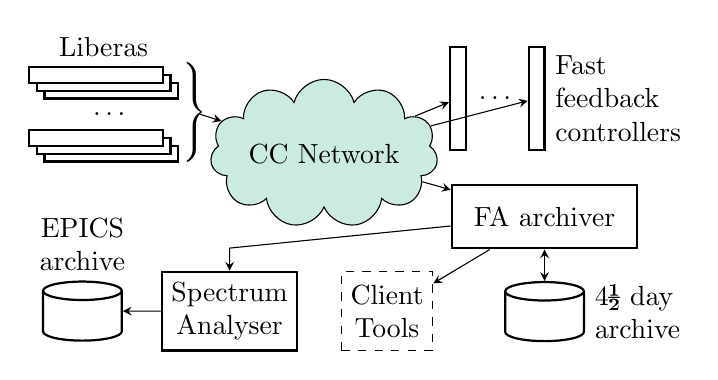
\begin{tikzpicture}

% Nice puffy cloud representing the FA network
\path[xshift=27mm, thin]
    node[draw, cloud, aspect=2, cloud puffs=11, inner sep=0pt, highlight fill]
        (fa network) {CC Network};

% Draw a stack of rectangles representing the liberas
\path[yshift=0.8cm,
    libera/.style={
        draw, rectangle, thick, fill=white, inner sep=0,
        minimum width=1.7cm, minimum height=2mm}]

    { [current point is local=true]
    node[libera] {}
    ++(-1mm,1mm) node[libera] {}
    ++(-1mm,1mm) node[libera] (top libera) {}
    }

    +(0mm,-3mm) node {\dots}
    ++(0mm,-8mm)
    { [current point is local=true]
    node[libera] (bottom libera) {}
    ++(-1mm,1mm) node[libera] {}
    ++(-1mm,1mm) node[libera] {}
    }
    node[tight fit=(top libera) (bottom libera),
        right delimiter=\}, label=north:Liberas] (liberas) {};

\draw[->] ($(liberas.east)+(2.6mm,0)$) -- (fa network);

% Fast feedback controllers
\path[yshift=7mm, xshift=44mm,
    controller/.style={
        draw, rectangle, thick, inner sep=0,
        minimum width=2mm, minimum height=13mm}]

    node[controller] (left controller) {}
    ++(5mm,0mm) node {\dots}
    ++(5mm,0mm) node[controller,
        label={[align=left]right:Fast\\feedback\\controllers}]
    (right controller) {};

\draw[->] (fa network) -- (left controller);
\draw[->] (fa network) -- (right controller);

% The archiver saving into the archive store
\path[xshift=5.5cm, yshift=-8mm]
    node[draw, thick, rectangle, inner sep=8pt]
        (archiver) {FA archiver}

    node[disk icon, below=4mm of archiver] (fa archive) {}
    node[tight fit=(fa archive),
        label={[align=left]right:4\textonehalf{} day\\archive}] {}
    [draw,<->] (archiver) -- (fa archive);

\draw[->] (fa network) -- (archiver);

% Spectrum analyser saving into EPICS archive
\path[xshift=15mm, yshift=-20mm]
    node[draw, thick, rectangle, align=center, minimum height=10mm]
        (spectrum) {Spectrum\\Analyser}

    node[disk icon, anchor=shape center,
        label={[align=center]above:EPICS\\archive}]
        (epics archive) at ($(spectrum.west)-(10mm,0)$) {}
    node[tight fit=(epics archive)] (epics archive fit) {}

    [draw,->] (spectrum) -- (epics archive fit);

\draw[->] (archiver) -- ($(spectrum)+(0,8mm)$) -- (spectrum);

% Client tools
\path[xshift=35mm, yshift=-20mm]
    node[draw, rectangle, align=center, minimum height=10mm, dashed]
        (client tools) {Client\\Tools};

\draw[->] (archiver) -- (client tools);

\end{tikzpicture}

\caption{FA Archiver and CC network in context.}
\label{context}
\end{figure}

The Communication Controller network was originally constructed to make the
10\,kHz FA data from each Libera BPM available for the operation of the fast
feedback controllers which maintain position stability of the electron beam.
The network synchronously distributes beam position $X$ and $Y$ coordinates
every 100\,\textmu s with a propagation delay of around 50\,\textmu s.

The design of the CC network with a highly redundant topology broadcasting by
storing and forwarding makes it easy to add new nodes to the network, both as
contributors and as passive listeners.  Other sources contributing to the
network are a handful of X-ray BPMs and power pick-ups from the RF cavities.
The FA archiver acts as a passive listener and makes the FA data freely
available.

The archiver stores data at the full data rate, referred to here as the ``FA''
rate, and at two decimated rates, ``D'' data decimated by a factor of 128, and
``DD'' ``double decimated'' data decimated by a factor of 16834.


\begin{figure*}[!ht]
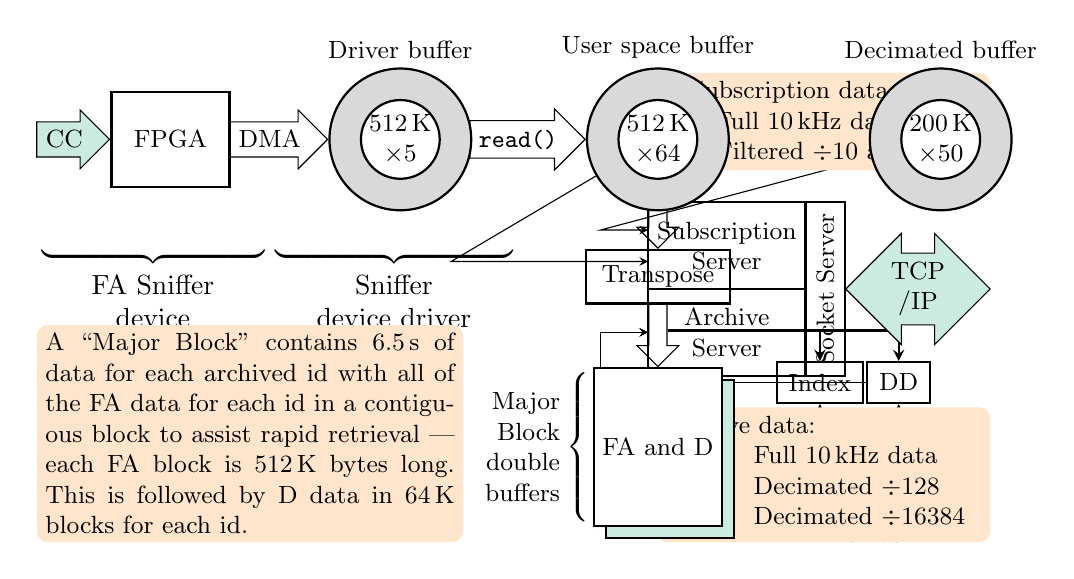
\begin{tikzpicture}[
    single arrow head extend=1.5mm]
\small

% Draws a circular buffer with name #1 east of #2 with top label #3 and centre
% label #4
\newcommand{\buffer}[4]{
\begin{pgfonlayer}{foreground}
\path
    node [draw, thick, circle, background fill,
        minimum width=18mm, anchor=west,
        label={above:#3}] (#1) at (#2.east) {}
    node [draw, thick, fill=white, circle, minimum width=10mm] at (#1) {}
    node [align=center, font=\small] at (#1) {#4};
\end{pgfonlayer}
}

% Sniffer device and its connections
\node [draw, single arrow, highlight fill, anchor=west] (cc) {CC};
\node at (0,-13mm) (anchor) {};
\node [draw, thick, anchor=west, minimum height=12mm, minimum width=15mm]
    (fpga) at (cc.east) {FPGA};
\node [draw, single arrow, anchor=west]
    (dma) at ($(fpga.east)-(0.2mm,0)$) {DMA};
\node [fit=(cc) (dma.center) (anchor-|dma.center),
    inner sep=0, below delimiter=\},
    label={[yshift=-3mm, font=\normalsize, align=center]below:
        FA Sniffer\\device}] {};

% Device driver
\buffer{device buffer}{dma}{Driver buffer}{512\,K\\$\times$5}
\node [draw, single arrow, anchor=west] at ($(device buffer.east)-(0.4mm,0)$)
    (device) {\texttt{read()}};
\node [fit=(dma.center) (device.center) (anchor-|dma.center),
    inner sep=0, below delimiter=\},
    label={[yshift=-3mm, font=\normalsize, align=center]below:
        Sniffer\\device driver}] {};

% Central raw circular buffer and decimated buffer
\buffer{raw buffer}{device}{User space buffer}{512\,K\\$\times$64}
\node [draw, single arrow, anchor=west] at ($(raw buffer.east)-(0.4mm,0)$)
    (decimate) {Decimate};
\buffer{decimated buffer}{decimate}{Decimated buffer}{200\,K\\$\times$50}


% Transposing to in-memory disk buffer
\node [draw, single arrow, rotate=-90, anchor=west, minimum height=5mm]
    (raw arrow) at ($(raw buffer.south)+(0,0.4mm)$) {};
\node [draw, thick, anchor=north, inner sep=2mm] at (raw arrow.east)
    (transpose) {Transpose};
\node [draw, single arrow, rotate=-90, anchor=west, minimum height=8mm]
    (transpose arrow) at ($(transpose.south)+(0,0.2mm)$) {};
\begin{pgfonlayer}{foreground}
\node [draw, thick, fill=white,
    minimum height=20mm, minimum width=15mm, anchor=north, align=center,
    left delimiter=\{, copy shadow={
        shadow xshift=1.5mm, shadow yshift=-1.5mm, highlight fill},
    label={[align=right, xshift=-3mm]left:Major\\Block\\double\\buffers}]
    (major block) at (transpose arrow.east) {FA and D};
\end{pgfonlayer}


% Archive on disk and in memory
\node [draw, single arrow, anchor=west, minimum width=1mm, minimum height=12mm,
    highlight fill]
    (archive arrow) at (major block.325) {};
\node [disk icon, anchor=west, label={below:Archive}]
    (archive) at (archive arrow.east) {};

\node [draw, thick, inner sep=1.5mm]
    (index) at ($(archive)+(-5mm,14mm)$) {Index};
\node [draw, thick, inner sep=1.5mm] (dd) at ($(archive)+(+5mm,14mm)$) {DD};

\draw [->, thick] (transpose arrow) -| (index);
\draw [->, thick] (transpose arrow) -| (dd);
\node [inner sep=0pt, line width=0] (via) at ($(archive.north)+(0,3mm)$) {};
\draw [<-, thick] (index) |- (via);
\draw [<->, thick] (dd) |- (via.center) -- (archive);

\node [right=5mm of via, align=center] {
    \scriptsize Memory\\[-1ex]\scriptsize mapped};


% Socket Server
\node [draw, double arrow, align=center, anchor=east, highlight fill]
    (tcp ip) at (\linewidth, -19mm) {TCP\\/IP};
\path [draw, thick]
    ($(tcp ip.west)-(0,11mm)$) rectangle ++(-5mm,22mm) coordinate (a)
    node [rotate=90, pos=0.5] {Socket Server}
    rectangle ++(-20mm,-11mm) coordinate (b)
    node [pos=0.5, align=center] {Subscription\\Server}
    rectangle ++(20mm,-11mm) coordinate (c)
    node [pos=0.5, align=center] {Archive\\Server}
    node [tight fit=(a) (b), align=center] (subscription server) {}
    node [tight fit=(b) (c), align=center] (archive server) {};

\draw [<-] ($(subscription server.west)+(0,-2mm)$)
    -- +(-25mm,0) -- (raw buffer);
\draw [<-] ($(subscription server.west)+(0,2mm)$)
    -- +(-6mm,0) -- (decimated buffer);
\draw [<-] (archive server.west) -- +(-6mm,0) |- (archive);
\draw [<-] (archive server.west) -- +(-6mm,0) |- (dd);


% Text boxes, key and major block description
\path coordinate (bottom) at ($(major block.south)+(0,-2mm)$) {};

\node [text fill, text width=37mm, anchor=south east]
    at ($(tcp ip.east |- subscription server.north)+(0,4mm)$) {
Subscription data:
\begin{itemize}[nolistsep, leftmargin=1em]
\item Full 10\,kHz data
\item Filtered $\div$10 at 1\,kHz
\end{itemize}};

\node [text fill, align=left, anchor=south east]
    at (tcp ip.east |- bottom) {
Archive data:\\
\begin{tabular}[t]{ll}
FA & Full 10\,kHz data \\
D & Decimated $\div$128 \\
DD & Decimated $\div$16384
\end{tabular}};

\node [text fill, text width=52mm, anchor=south west, align=justify]
    at (cc.west |- bottom) {
A ``Major Block'' contains 6.5\,s of data for each archived id with all of the
FA data for each id in a contiguous block to assist rapid retrieval --- each FA
block is 512\,K bytes long.  This is followed by D data in 64\,K blocks for each
id.
};

\end{tikzpicture}

\caption{Architecture of FA archiver showing device, driver and archiver process
writing to disk and serving clients.}
\label{architecture}
\end{figure*}


\section{Archiver Architecture}

The FA archiver consists of the following components:
\begin{description}[noitemsep]

\item[FA Sniffer.]  This is an implementation of the Communication Controller on
a Virtex-5 FPGA PCI Express (PCIe) board. The sniffer captures communication
frames and transfers them by DMA to memory.

\item[Sniffer device driver.]  The device driver communicates with the sniffer
card and makes the data stream available as a Linux device node,
\texttt{\small/dev/fa\_sniffer0}.

\item[Archiver process.]  The archiver process reads frames from the device
driver, saves them to disk after processing to optimise subsequent reading, and
provides a socket server for client access to both the live data stream and a
$\div10$ decimated stream.

\item[Client tools.]  A variety of client tools are able to connect directly to
the archiver server, including a data visualisation tool (\texttt{fa-viewer})
for viewing the live data, a general purpose command line tool
(\texttt{fa-capture}) for reading from the archive, and a Matlab script
(\texttt{fa\_zoomer}) for exploring the archive.

\end{description}


\subsection{FA Sniffer}

\begin{figure}[ht]
\centering
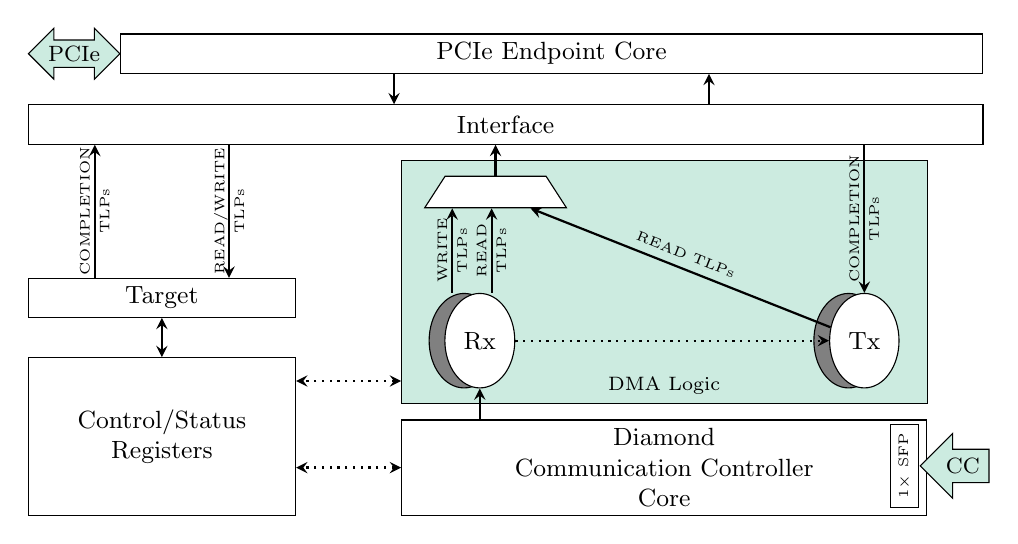
\begin{tikzpicture}[
    interface/.style={draw, minimum width=\linewidth, minimum height=5mm},
    left module/.style={draw, minimum width=0.28\linewidth, align=center},
    right module/.style={draw, minimum width=0.55\linewidth, align=center},
    buffer/.style={draw, fill=white, ellipse, minimum height=12mm,
        copy shadow={shadow xshift=-2mm, shadow yshift=0, shadow fill}}]
\small

% External interface: endpoint core and internal interface
\node[draw, double arrow, highlight fill, anchor=west,
    double arrow head extend=1.5mm, inner sep=2pt]
    (pcie) {\footnotesize PCIe};
\path[draw] ($(pcie.east)+(0,-2.5mm)$) rectangle (\linewidth,2.5mm)
    node[pos=0.5] (pcie core) {PCIe Endpoint Core};
\node[interface, anchor=west] at (0,-9mm) (interface) {Interface};

\draw[thick, ->, transform canvas={xshift=-20mm}]
    (pcie core) -- (interface.north -| pcie core);
\draw[thick, <-, transform canvas={xshift=20mm}]
    (pcie core) -- (interface.north -| pcie core);


% Internal control modules: register interface
\node[left module, anchor=west, yshift=-22mm] at (interface.west)
    (target) {Target};
\node[left module, below=5mm of target, minimum height=20mm]
    (registers) {Control/Status\\Registers};

\draw[thick, ->]
    ($(target.north west)!.25!(target.north east)$) node (start) {} --
        (start |- interface.south)
    node[pos=0.5, sloped, align=center] {\tiny COMPLETION\\[-1ex]\tiny TLPs};
\draw[thick, <-]
    ($(target.north west)!.75!(target.north east)$) node (start) {} --
        (start |- interface.south)
    node[pos=0.5, sloped, align=center] {\tiny READ/WRITE\\[-1ex]\tiny TLPs};
\draw[thick, <->] (target) -- (registers);


% Communication controller core and its SFP
\node[right module, anchor=south east, xshift=\linewidth-7mm]
    at (registers.south west)
    (cc core) {Diamond\\Communication Controller\\Core};
\node[draw, rotate=90, anchor=south west, xshift=1mm, yshift=1mm,
    minimum width=10mm]
    at (cc core.south east)
    (sfp) {\tiny 1$\times$ SFP};
\node[draw, single arrow, shape border rotate=180,
    single arrow head extend=2mm,
    anchor=west, highlight fill]
    at (sfp.south) {\footnotesize CC};


% Background for the big DMA engine in the middle
\path[draw, highlight fill]
    ($(cc core.north east)+(0,2mm)$) coordinate (dma se) {}
    ($(interface.south -| cc core.east)-(0,2mm)$) coordinate (dma ne) {}
    rectangle (dma se -| cc core.west) coordinate (dma sw) {}
    (dma sw |- dma ne) coordinate (dma nw) {};
\path (dma sw) -- (dma se)
    node[pos=0.5, above] {\scriptsize DMA Logic};

% Buffers and multiplexor in DMA engine
\node[draw, fill=white, trapezium, minimum height=4mm, minimum width=18mm,
    trapezium stretches body=true, trapezium angle=40]
    at ($(dma nw)+(12mm,-4mm)$) (mux) {};
\node[buffer] at ($(dma sw)+(10mm,8mm)$) (rx buf) {Rx};
\node[buffer] at ($(dma se)+(-8mm,8mm)$) (tx buf) {Tx};


\draw[thick, ->, dotted] (rx buf) -- (tx buf);
\draw[thick, ->] (tx buf) -- (mux.335)
    node[pos=0.5, sloped, above] {\tiny READ TLPs};
\draw[thick, ->, transform canvas={xshift=1.5mm}]
    (rx buf.north) -- (rx buf.north |- mux.south)
    node[pos=0.5, sloped, align=center] {\tiny READ\\[-1ex]\tiny TLPs};
\draw[thick, ->, transform canvas={xshift=-3.5mm}]
    (rx buf.north) -- (rx buf.north |- mux.south)
    node[pos=0.5, sloped, align=center] {\tiny WRITE\\[-1ex]\tiny TLPs};

\draw[thick, ->] (mux) -- (mux |- interface.south);
\draw[thick, ->] (tx buf |- interface.south) -- (tx buf)
    node[pos=0.5, sloped, rotate=180, align=center]
    {\tiny COMPLETION\\[-1ex]\tiny TLPs};


\draw[thick, ->] (cc core.north -| rx buf) -- (rx buf);
\draw[<->, dotted, thick] (cc core) -- (cc core -| registers.east);
\draw[<->, dotted, thick, transform canvas={yshift=11mm}]
    (cc core) -- (cc core -| registers.east);
\end{tikzpicture}

\caption{Architecture of the FA sniffer FPGA.}
\label{fa-sniffer}
\end{figure}

The FA Sniffer is so called because it passively ``sniffs'' FA data from the
communication controller network.  The FPGA design integrates the Diamond
Communication Controller~\cite{cc} into a bus master PCI Express architecture
using the commercially available Xilinx Virtex-5 FPGA ML555 development
platform~\cite{fpga-kit}.  The design consists of target logic, DMA initiator
logic, status/control registers and the Virtex-5 endpoint core for PCI Express.
Target logic is responsible for capturing single double-word memory write and
memory read PCIe Transaction Layer Packets (TLPs) for control and status
register access.  The DMA initiator logic generates memory write TLPs to
transfer 2\,K byte frame data from the communication controller core to the
host's system memory.  The complete design occupies 30\,\% of bit slices and
20\,\% of block RAMs available on the FPGA.

The communication controller core captures a complete frame from the CC network
on every communication controller cycle, with a new cycle starting every
100\,\textmu s.  The frame transferred to memory by the sniffer is 2048 bytes
consisting of 256 samples, each a pair of four-byte numbers corresponding to
measured $X$ and $Y$ positions for FA ids 1--255 together with a 32-bit
timestamp counter repeated in position 0 as ``id 0''.

The sniffer card maintains a queue of up to two DMA targets, address and frame
count, one being written to, the next to be loaded when the first target is
filled, at which point an interrupt is raised to the host machine.  At this
point the device driver is responsible for setting up a fresh buffered DMA
target, otherwise the sniffer will halt.


\begin{figure}[ht]
\centering
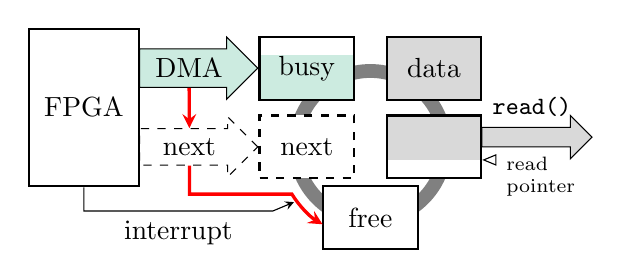
\begin{tikzpicture}[
    single arrow head extend=1.5mm,
    buffer/.style={draw, thick, minimum width=12mm, minimum height=8mm}]

\node [draw, thick, anchor=west, minimum height=20mm, minimum width=14mm]
    (fpga) {FPGA};

\node [draw, highlight fill, single arrow, anchor=west, minimum height=15mm]
    (dma) at ($(fpga.east)+(-0.4pt,5mm)$) {DMA};
\node [draw, dashed, single arrow, anchor=west, minimum height=15mm]
    (next) at ($(fpga.east)+(-0.4pt,-5mm)$) {next};

\node [buffer, anchor=west]
    (dma buf) at (dma.east) {busy};
\node [buffer, fill=white, dashed, anchor=west]
    (next buf) at (next.east) {next};
\node [buffer, xshift=10mm, background fill]
    (data buf1) at (dma buf.east) {data};
\node [buffer, xshift=10mm] (data buf2) at (next buf.east) {};
\node [buffer, fill=white, anchor=center, yshift=-9mm]
    (free) at ($(next buf)!.5!(data buf2)$) {free};

\node [draw, isosceles triangle, rotate=180, anchor=east, inner sep=1pt,
    label={[align=left, font=\scriptsize, yshift=2mm]above left:read\\pointer}]
    (marker) at ($(data buf2.south east)!0.3!(data buf2.north east)$) {};

\node [draw, single arrow, background fill, anchor=west, minimum height=14mm,
    label={above:\small\texttt{read()}}]
    at ($(marker.east)!.5!(data buf2.north east)-(0.4pt,0)$) {};


\begin{pgfonlayer}{background}
\node [line width=5pt, draw=gray, circle, minimum size=19mm]
    (circle) at ($(next buf.north east)!.5!(data buf2.north west)-(0,4mm)$) {};
\path [fill=white]
    (data buf2.north west) rectangle (data buf2.south east);
\path [highlight fill]
    (dma buf.south west) rectangle
    ($(dma buf.north east)!.3!(dma buf.south east)$);
\path [background fill]
    (data buf2.north west) rectangle (marker.east);
\end{pgfonlayer}

\path [->, draw=red, color=red, very thick] (dma) -- (next);
\path [->, draw=red, color=red, very thick]
    (next) -- ++(0,-6mm) -- +(13mm,0) arc (212:239:11.7mm);

\draw[->]
    (fpga.south) -- ++(0,-3mm) -- ++(24mm,0)
    node[pos=0.5, below] {\smash[b]{interrupt}}
    -- ($(circle.215)-(1.2mm,1.2mm)$);

\end{tikzpicture}

\caption{Architecture of the sniffer device driver.}
\label{driver}
\end{figure}

\subsection{Sniffer Device Driver}

The sniffer device driver maintains a circular pool of buffers for the FA
sniffer to write to, by default five buffers of 512\,K bytes each, enough
storage for 40\,ms of data per buffer.  When the sniffer is running, two buffers
are allocated to the sniffer and the remaining buffers contain data for the
user space program to read or are free for the next DMA transfer.  On each
interrupt the pool cycles round by one buffer unless there is no free buffer, in
which case the sniffer is allowed to halt.

Data capture is also interrupted during CC network synchronisation or if a
communcation error occurs.  Any interruption is signalled by the driver as ``end
of file'' and recorded by the archiver as a gap in the archive.


\subsection{The Archive on Disk}

\begin{figure}[ht]
% Disk layout

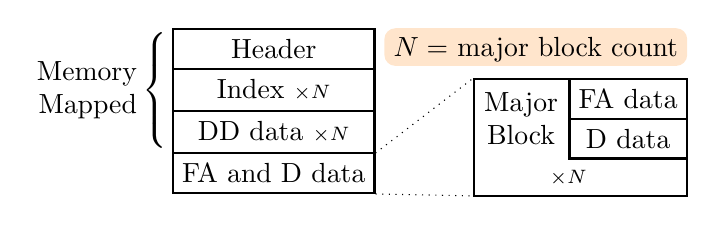
\begin{tikzpicture}

\node [draw, thick, rectangle split, rectangle split horizontal=false]
    (disk layout)
{
    Header
\nodepart{two}
    Index {\scriptsize $\times N$}
\nodepart{three}
    DD data {\scriptsize $\times N$}
\nodepart{four}
    FA and D data
};

\node [tight fit=(disk layout.north west) (disk layout.three split west),
    left delimiter=\{,
    label={[align=right, xshift=-2ex]left:Memory\\Mapped}] {};

\path[draw, thick]
    node [draw, thick, rectangle split, rectangle split horizontal=false,
        rectangle split parts=2] (fa layout) at (45mm,-1mm)
        {FA data \nodepart{two} D data}

    node [anchor=east, align=center]
        (major block) at (fa layout.west) {Major\\Block}
    node [anchor=north] at (fa layout.south west)
        (by N) {\scriptsize $\times N$}
    ($(fa layout.north east)-(0.4pt,0.4pt)$)
    rectangle (by N.south -| major block.west);

\draw[dotted]
    (disk layout.south east) -- (by N.south -| major block.west)
    (disk layout.three split east) -- (major block.west |- fa layout.north);

\node[text fill, anchor=north east] at (fa layout.east |- disk layout.north)
    % We smash away the descender on j to improve the look of the enclosing box.
    {$N=$ \smash[b]{major block count}};

\end{tikzpicture}

\smallskip
Per major block, repeated for each archived FA id:
\smallskip

\begin{tabular}[t]{l>{$}l<{$}>{$}l<{$}}
FA data: & \begin{array}{l}x,y\end{array} & \times 65536 \\
D/DD data: &
\begin{array}{l}
\overline{x}, \overline{y}, \lfloor x\rfloor, \lfloor y\rfloor, \\
\lceil x\rceil, \lceil y\rceil, \sigma_x, \sigma_y
\end{array}
& \times 512/ \mathord\times 4
\end{tabular}

\caption{Layout of archive store on disk.}
\label{fa-layout}
\end{figure}


The FA data stream from the sniffer is uniform, with constant sized updates
received at an unchanging interval.  The only variation in this structure is the
occasional presence of gaps in the data stream where synchronisation of the
communication network has been performed.

This uniform data format allows the archive to be stored as a simple
fixed-format file.  For performance it is better for the archive to be stored
directly on the underlying block device, as the filesystem block management
otherwise adds a significant overhead for very large files.

Early experiments with the archive revealed that the optimum block size for
transfers to and from disk is around 512\,K bytes and so the layout of the
archive on disk is optimised for reading by placing the data for a single FA
identifier into blocks of 512\,K bytes or 65536 samples each, or around
6\textonehalf{} seconds of data.

At the same time, to help with generating an overview of the entire archive,
data is binned into 128 and 16384 sample bins in which the mean, minimum,
maximum, and standard deviation values are computed.  The decimated $\div$128
data is stored together with the FA data as a ``major block'', the $\div$16384
data is stored separately in a memory mapped area.

These major blocks are indexed by timestamps recorded in the index which is
searched by binary search when an archive read request is processed.

A fixed size (4096 byte) header defines all of the operating parameters of the
archiver (block sizes, decimation factors, etc.) together with the list of FA
ids archived, and also records the current active block.

\subsection{Data Processing}

Two major blocks are maintained in memory, one being prepared as frames are
received from the FA sniffer, the other being written to disk.  FA sniffer
frames are transposed (in blocks of 256 frames) into the major block layout.

To ensure that reads from the archive do not delay writes there is a limit on
the number of reads that can be requested simultaneously, and there is also an
interlock to prevent a read being initiated while writing to disk is in
progress.


\subsection{Filtered Decimation}

For some applications of the archiver live FA data feed at the full 10\,kHz data
rate is too much; for example most of the environmental disturbances on the beam
have their main effects in the bottom few hundred Hertz.  In particular, the
full orbit Spectrum Analyser (described below) only covers frequencies up to
320\,Hz.

Thus the archiver decimates the full FA data by a factor of 10 using a
compensated CIC filter~\cite{hogenauer, altera}, and this data stream is
available as an alternative data source for subscribers.  The spectrum of the
decimated data is flat to $\pm0.25$\,dB with better than 100\,dB alias rejection
up to 350\,Hz.


\section{Applications}


\subsubsection{Archive Retrieval.}

A command line tool \texttt{fa-capture} provides full access from the command
line to the dataset stored on the FA archiver, allowing any part of the archive
to be retrieved and saved in either raw or Matlab format.  Start and end times
or start and sample count can be specified in a variety of formats.

\subsubsection{Archive Exploration in Matlab.}

A Matlab tool called the \texttt{fa\_zoomer} allows the archive to be explored
interactively.  An interactive window displays the current selection and allows
any part of the selection to be zoomed and retrieved in more detail from the
archive.  The initial window uses ``double decimated'' data to show an overview
of either the last 24 hours or the entire available archive (4\textonehalf{}
days), and the decimation is reduced as zooming is refined.

% Note that \linewidth has the right behaviour here, and automatically picks up
% the right size if we go for a double width figure with figure*.  The
% alternatives appear to be \columnwidth and \textwidth.
\begin{figure}[ht]
\centering
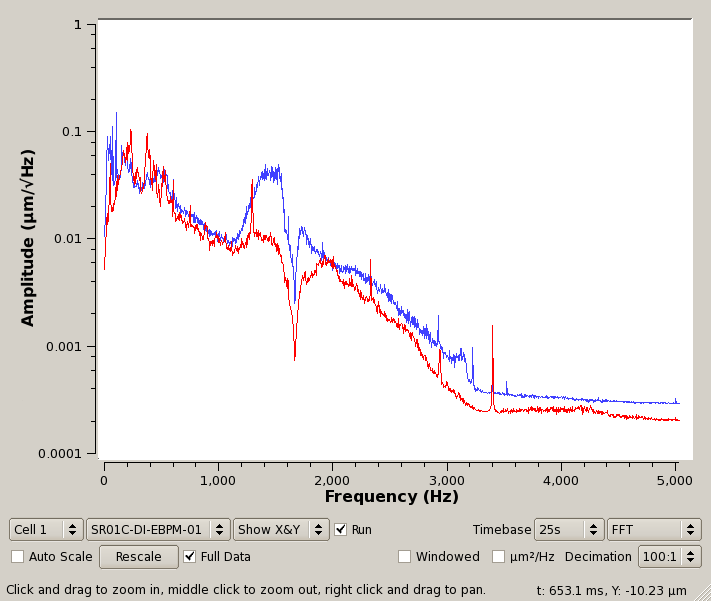
\includegraphics[width=\linewidth]{THCHMUST03f6}
\caption{FA viewer application showing beam motion power spectrum of selected
BPM over the last 25 seconds.}
\label{fa-zoomer}
\end{figure}

\subsubsection{Live Visualisation.}

The \texttt{fa-viewer} tool is a Python Qt application used to visualise the
motion of the beam at any chosen single location.  The user can choose to
observe any available FA identifier which is then displayed as either a live
history display (for up to 60 seconds of history) or a variety of spectral
displays: FFT on log y or log xy scales, or an integrated power spectrum.
Graphing is done using PyQwt~\cite{pyqwt} which is both fast and flexible,
making it straightforward to develop a large variety of visualisations.

\subsubsection{Audio Playback.}

As the beam disturbance frequencies as processed by the FA archiver are
comfortably audible it was natural to try playing back the beam position as
sounds.  This turns out to work very well, and is occasionally quite
instructive.  Both topup and injection have very distinctive sounds, but what is
more interesting is the variety of very odd sounds that appear to be
superimposed on the beam by disturbances in the RF system.

\subsubsection{Long Term Spectral Analysis.}

A dedicated server subscribes to the 1\,kHz complete live orbit data and
computes averaged power spectra in 1\,Hz bins averaged every five minutes
covering the spectral range from 1 to 320\,Hz.  Complete waveforms for all
frequencies and all 174 BPMs are generated as EPICS PVs, both as power density
spectra for each BPM and orbit disturbance for each frequency, and a limited
selection of these waveforms is archived in the long term EPICS archive.

This allows a detailed examination of changes in the spectral behaviour of the
machine over extended periods; it is easy to look at the
spectrum for a week's operation of the machine and identify long term changes in
disturbance.

\subsubsection{Other Users.}

The sources for the archiver and driver can be downloaded from the Diamond web
site~\cite{download}, and the FA archiver has been used at Soleil since May
2011.


\section{Conclusions}

The motivation for the FA Archiver has been to gain access to longer periods of
synchronously recorded position data from all channels (the whole orbit) at FA
data rate. Previously our setup had only been able to capture ten seconds of
this data using buffers inside the fast feedback processors.  Having access to
records of up to several days of this data facilitates the following:

\begin{itemize}

\item Identification and detailed investigation of any orbit events that
happened in the recent past.  To this end, the maximum/minimum/standard
deviation calculations on the $\div$16384 decimated data are invaluable.

\item Correlation of orbit events with other measurements by adding X-ray BPMs
and RF cavity voltage readings to the FA network~\cite{rehm}.

\item Modal analysis of orbit motion over longer periods. This is useful for the
optimisation of the fast orbit feedback and for the identification of BPMs or
correctors with subtle malfunctions.

\end{itemize}

Together with the long term spectral analysis all these methods allow monitoring
and improvement of the reliability and performance of the fast orbit feedback
system and ultimately the beam stability.



\begin{thebibliography}{99}

\bibitem{i-tech}
Instrumentation Technologies, \url{http://www.i-tech.si}.

\bibitem{control-system}
M.G.~Abbott, G.~Rehm, I.S.~Uzun, ``The Diamond Light Source Control System
Interface to the Libera Electron Beam Position Monitors'', ICALEPCS 2009.

\bibitem{cc}
I.S.~Uzun, R.~Bartolini, G.~Rehm, J.A.~Dobbing, M.T~Heron, J.~Rowland, ``Initial
Design of the Fast Orbit Feedback System for Diamond Light Source'', ICALEPCS
2005

\bibitem{fast-feedback}
M.G.~Abbott, J.A.~Dobbing, M.T.~Heron, G.~Rehm, J.~Rowland, I.S.~Uzun,
S.~Duncan, ``Diamond Light Source Electron Beam Position Feedback: Design,
Realization and Performance'', ICALEPCS 2009.

\bibitem{fpga-kit}
Virtex-5 LXT ML555 FPGA Development Kit for PCI Express,
\url{http://www.xilinx.com/products/boards-and-kits/HW-V5-ML555-G.htm}

\bibitem{hogenauer}
E.B.~Hogenauer, ``An economical class of digital filters for decimation and
interpolation'', IEEE Transactions on Acoustics, Speech and Signal Processing,
pp.~155--162, April 1981

\bibitem{altera}
Altera Corporation, ``Understanding CIC Compensation Filters'', AN-455-1.0,
\url{www.altera.com/literature/an/an455.pdf}

\bibitem{pyqwt}
\url{http://pyqwt.sourceforge.net/}

\bibitem{download}
\url{http://controls.diamond.ac.uk/downloads/other/fa-archiver}

\bibitem{rehm}
G.~Rehm, M.G.~Abbott, C.~Bloomer, I.~Uzun,  ``Synchronous Measurement of
Stability of Electron Beam, X-Ray Beam, Ground and Cavity Voltage'', DIPAC'11


\end{thebibliography}


\end{document}
